%!TEX root = ../main.tex

\chapter{Introduction}
\label{chp:intro}

\section{The non-terrestrial era}
The \ac{3GPP}\footnote{\href{https://www.3gpp.org}{\texttt{3gpp.org}}}, the standardization body tasked with the development of protocols for mobile communication networks, recently put a great emphasis on the importance of the integration of different access technologies along with the existing terrestrial mobile telecommunication infrastructure \cite{3gpp-tr-21.917}.

Specifically, the envisioned future for mobile communications, starting with the already established 5G \ac{NR} and further expanding with the new sixth-generation cellular networks (6G), foresees the integration of a new non-terrestrial component. The latest \ac{3GPP} releases (Rel. 17 and Rel. 18) require 5G and 6G networks to be able to provide non-terrestrial satellite access complementing the already existing terrestrial access technologies \cite{overview-rel-17-18-saad, 5g-nr-communication-geo-leo-maattanen}.

To give a proper definition, the term \ac{NTNs} refers to a category of networks where at least one link is routed via an aerial or space-borne vehicle such as \ac{HAPs}, \ac{UAVs} or telecommunication satellites.

\section{Limitations of terrestrial networks}
In order to explain the motivations behind the choice of expanding the current terrestrial infrastructure, the following sections present a few scenarios where the current terrestrial infrastructure fails to provide an adequate service due to some of their intrinsic limitations, and \ac{NTNs} can help to provide a better coverage.

\begin{figure}[ht]
    \centering
    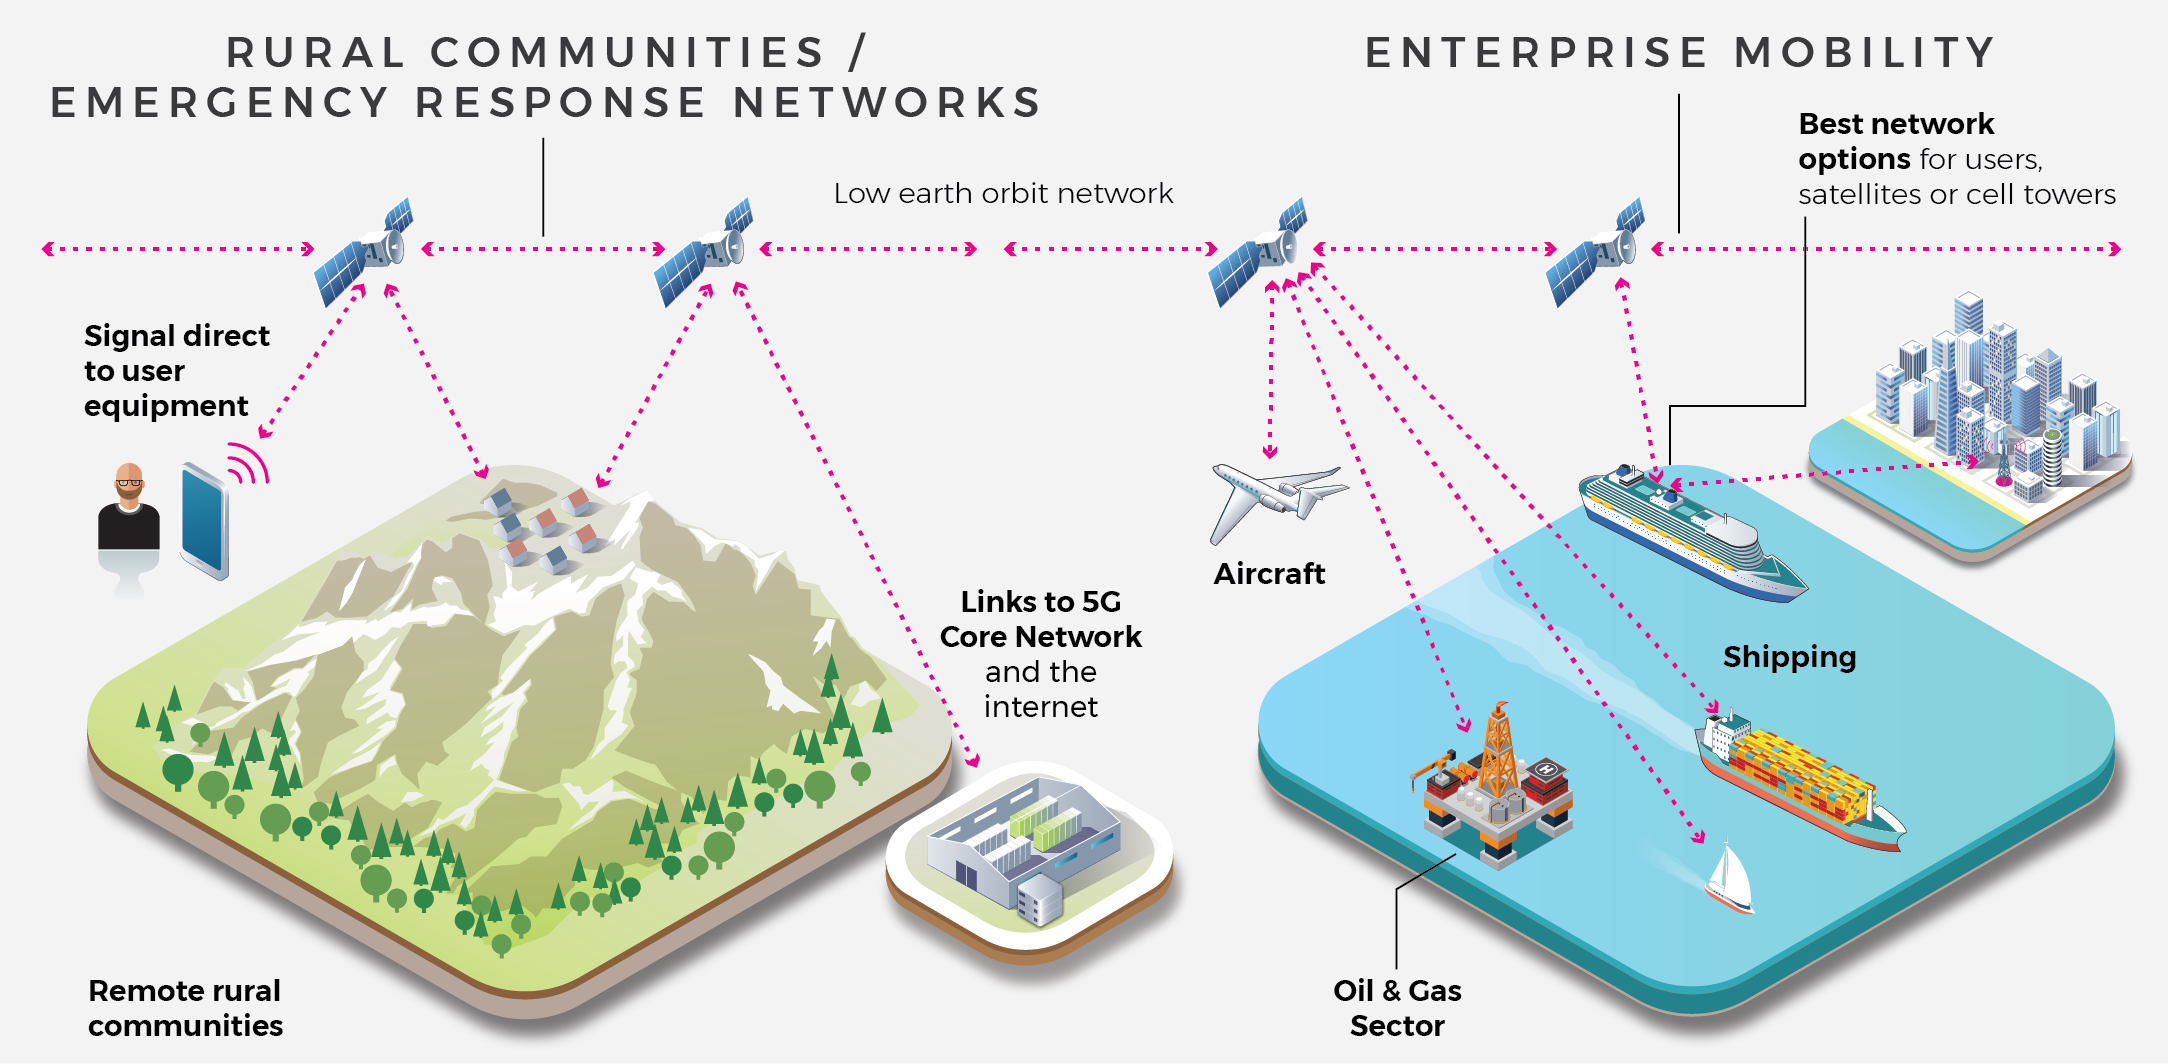
\includegraphics[width=0.9\textwidth]{res/sat-usecases.png}
    \caption{NTN use cases, courtesy of \href{https://telecominfraproject.com/ntcs/}{telecominfraproject.com}}
    \label{fig:sat-use-cases}
\end{figure}

\subsection{Remote places}
While \ac{TN} make the well-established foundation of today’s mobile communication infrastructure, their own nature poses some intrinsic limitations to their deployment in certain scenarios, especially in contexts of rural and remote areas. Conditions such as harsh terrain and geographical impediments like mountain ranges and large bodies of water act as natural barriers to the deployment of terrestrial infrastructure. Moreover, the need for ground equipments such as base stations and networking gear requires the presence of an already established and reliable power grid, further driving up the costs that telecommunication companies would have to sustain to bring connectivity in isolated areas without such amenities.

\paragraph{Population density}
The population density in remote and rural places is typically much lower than the one found in cities, and users are spaced in vast areas of land. Because of this reason, the investment that has to be made on a per-user basis in order to provide coverage would be much higher compared to a more urbanized scenario, where potential users are more densely distributed. The already high infrastructure cost will therefore have a hard time generating any profit, making this kind of market even more unattractive to private investors and further limiting the possibility for the people living there to access the internet, a resource which is becoming increasingly more important as time goes by.

\paragraph{Opportunities}
As studied and documented in \cite{6g-challenge-opportunity-base-pyramid}, the issue of an inadequate broadband coverage in rural regions is an enormous challenge. Providing connectivity to the half of the world population living in rural or underprivileged areas requires a colossal effort, but it would also be a unique opportunity to kick-start the economy of currently underdeveloped countries. Access to the Internet would provide the population a possibility to progress on the educational, environmental, business and health planes, promoting a more fair access to information and alleviating the problem of digital divide between different parts of the world.

\subsection{Redundancy and additional capacity}
Another limitation of the current terrestrial infrastructure is the lack of redundancy and robustness against natural disasters. Extreme events such as earthquakes, hurricanes, fires and floods, but also deliberate behaviors such as targeted attacks by terrorist organizations and sabotages can disrupt the connectivity, leading to outages that can potentially last for a long period of time. This in turn can cause significant economical damage and, in emergency situations, hinder the already difficult rescue efforts, potentially even leading to loss of lives.

The simple installation of additional base stations is not a viable solution because they would all share the same weaknesses, and extreme events such as tornados would easily be able to render all the additional equipment useless. The cost of essentially doubling the existing access network to make it more resilient would be enormous.

In this scenario, \ac{NTNs} can act as a redundant access methodology to decrease the downtimes of terrestrial infrastructure, providing emergency communication services as well as additional capacity when required.

Fig. \ref{fig:multiple-connectivity}, courtesy of \cite{3gpp-tr-38.811}, shows a scenario where terrestrial and non-terrestrial access technologies are used transparently to access the network. It depicts a \ac{UE} that can use both the non-terrestrial link provided by the satellite or the terrestrial one. In this case, the satellite is connected to a ground gateway where the \ac{gNB} is located, therefore only rerouting the signal coming from the \ac{UE}.

\begin{figure}[ht]
    \centering
    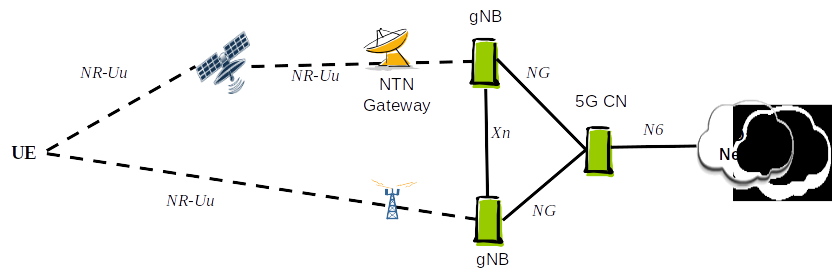
\includegraphics[width=0.7\textwidth]{res/multiple-connectivity.png}
    \caption{Transparent use of multiple radio access technology \cite{3gpp-tr-38.811}}
    \label{fig:multiple-connectivity}
\end{figure}

\subsection{Long distances and sensors}
Remote equipment, offshore plants and distribution grids will also benefit from the research carried out in this field, since providing terrestrial connectivity in those scenarios is a very challenging task due to the physically long distances involved. The installation of an underwater optical fiber link to serve a single endpoint, such as an offshore oil rig or power plant located in the open ocean, would bear a disproportional cost compared to the functions required, and providing maintenance would be another challenging and expensive task. 
The deployment of non-terrestrial networks would be the easiest way to provide connectivity on a global scale, therefore allowing internet access in isolated places without the need for an expensive, dedicated connection.

Consider now the problem of connecting a number of sensors sparsely distributed in a large area. When distances are large, solutions may be either the densification of radio stations or the use of a lower frequency in order to have a less severe propagation loss. However, those approaches have their downsides and are not always feasible, requiring costly, ad-hoc solutions tailored for each specific scenario. In this case, the vast coverage area of \ac{NTNs} will undoubtedly be useful to provide internet connection \cite{performance-ntn-support-iot-wang}.

\paragraph{} Other scenarios where \ac{NTNs} can become useful in overcoming the limitation of their terrestrial counterpart are well described in \cite{ntn-6g-era-challenges-giordani} and \cite{potential-multilayered-nierarchical-ntn-wang}.


\section{Structure of this work}

The main objective of this thesis is the use of a full stack end to end network simulator to evaluate the problems with the current implementation of 5G \ac{NR} protocol stack when confronted with the non-terrestrial scenario characterized by a high propagation delay, studying their behaviors as well as presenting some original proposals and solutions that will allow communication to take place.

\paragraph{}
After the above introduction, the second chapter (\ref{chp:ntn}) consists of a deep dive into the realm of non-terrestrial networks, resulting from a comprehensive review of the current state of the art. The three main categories of telecommunication satellites are described, and their characteristics evaluated. Finally, an overview of the possible payload design choices is presented, discussing advantages and disadvantages, as well as a brief description of the potential of multilayered networks.

\paragraph{}
The focus then shifts to ns-3, the employed network simulator software, highlighting the NTN channel module used as well as its implementation, and detailing the reasons behind its choice. Finally, emphasis is put on presenting the simulated scenario, describing the characteristics and the parameters of all the involved devices.

\paragraph{}
After this initial presentation and characterization of the used tools, chapter \ref{chp:scheduling_problems} is about the scheduler. The 5G scheduler and its operations in time division duplexing are briefly described, then the main design flaws that arose during the simulations in non-terrestrial scenarios are documented, and the implemented solutions are carefully explained. 

In particular, the scheduler was modified to schedule resources with more advance to account for the additional delay, and to expect a non-immediate \ac{UE} response, a behavior that was not considered in the standard implementation.

A problem regarding the expiration of buffer status reports also arose, leading to wasted resources since the \ac{UE} essentially flooded the base station with unnecessary requests. A modification was implemented to the \ac{UE} so that it waits for at least a full round-trip time before trying to send a new request.

The standard implementation of the \ac{UE} MAC protocol is configured in such a way that each incoming packet triggers a scheduling request for the full transmission buffer, regardless of previous requests that may still be in transit, therefore wasting capacity. The implementation of a less aggressive mechanism managed to increase the efficiency.


\paragraph{}
Then, moving up in the ladder of protocol layers, the problems related to the operation of HARQ in a non-terrestrial scenario are presented, discussing the effects of propagation delay as well as the impact of different values of SNR, linked to the satellite orbiting altitude and \ac{UE} antenna. Some solutions are proposed and evaluated using the ns-3 network simulator.

The maximum number of concurrent processes that \ac{NR} implementation enforces is found to be a major limiting factor for the throughput, therefore its increase has been evaluated, and, while this managed to increase the achievable throughput, its effects were limited when compared with the additional complexity that such approach would require.

Simulations performed without HARQ showed that better results could be obtained, but this solution only works in conditions with high SNR, therefore a more aggressive version of HARQ is presented, aimed at lowering the impact of the limited amount of concurrent processes.

\paragraph{}
Finally, the conclusions of this thesis are presented, highlighting how scheduler and HARQ are affected by the characteristics of a non-terrestrial link, summarizing all the obtained results as well as the proposed solutions, and providing some paths that can be explored in future studies.